\section{Definición del Problema}

\begin{frame}{El entorno Mountain Car Continous (MCC)}
    \begin{columns}[T,onlytextwidth]
        % ---- Columna izquierda: texto ----
        \column{0.55\textwidth}
        \begin{itemize}
            \item \textbf{Objetivo}: alcanzar la cima
            \item \textbf{Dificultad}: el agente debe aprender a balancearse
            \item \textbf{Espacio de Estados}:
                \begin{itemize}
                    \item Posición: $p \in \left[ -1.2 , 0.6 \right]$
                    \item Velocidad: $v \in \left[-0.07, 0.07 \right]$
                \end{itemize}
            \item \textbf{Espacio de Acciones}:
                \begin{itemize}
                    \item Fuerza de empuje: $f \in \left[-1,1\right]$
                \end{itemize}
            \item \textbf{Actualización}:
                \begin{itemize}
                    \item $velocidad_{t+1} = velocidad_t + fuerza \cdot 0.0015 - 0.0025 \cdot \cos(3\cdot posicion_t)$.
                    \item $posicion_{t+1} = posicion_t +velocidad_{t+1}$
                \end{itemize}
        \end{itemize}
        % ---- Columna derecha: imagen ----
        \column{0.45\textwidth}
        \begin{center}
        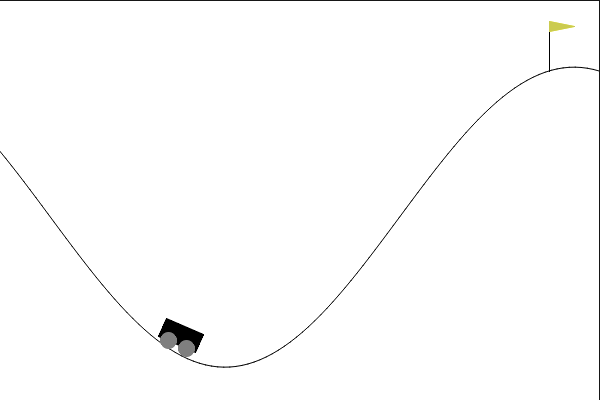
\includegraphics[
            width=0.8\linewidth,
            height=0.70\textheight,
            keepaspectratio
        ]{./attatchments/mcc.png}
        \end{center}
  \end{columns}
\end{frame}

\begin{frame}{El entorno Mountain Car Continous (MCC)}
    \begin{columns}[T,onlytextwidth]
        % ---- Columna izquierda: texto ----
        \column{0.55\textwidth}
        \textbf{Funcion de recompensa}
        \begin{itemize}
            \item \textbf{Bonificación por Éxito:} llegar a meta ($p \geq 0.45$)  $$r_{t+1} = 100$$.
            \item \textbf{Penalización por Esfuerzo:} En cada paso donde no se alcanza la meta $$r_t = -0.1 \cdot a_t^2$$.
        \end{itemize}
        % ---- Columna derecha: imagen ----
        \column{0.45\textwidth}
        \begin{center}
        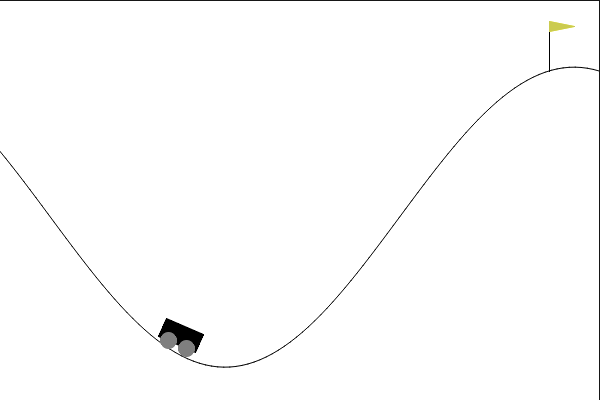
\includegraphics[
            width=0.8\linewidth,
            height=0.70\textheight,
            keepaspectratio
        ]{./attatchments/mcc.png}
        \end{center}
  \end{columns}
\end{frame}